% Use only LaTeX2e, calling the article.cls class and 12-point type.

\documentclass[12pt]{article}

% Users of the {thebibliography} environment or BibTeX should use the
% scicite.sty package, downloadable from *Science* at
% http://www.sciencemag.org/authors/preparing-manuscripts-using-latex
% This package should properly format in-text
% reference calls and reference-list numbers.

\usepackage{scicite}

\usepackage{times}

% Packages I manually added
\usepackage{graphicx}
\usepackage{placeins}
\usepackage{float}
\usepackage{amsmath}
\usepackage{hyperref}
\usepackage{pdflscape}



% The preamble here sets up a lot of new/revised commands and
% environments.  It's annoying, but please do *not* try to strip these
% out into a separate .sty file (which could lead to the loss of some
% information when we convert the file to other formats).  Instead, keep
% them in the preamble of your main LaTeX source file.


% The following parameters seem to provide a reasonable page setup.

\topmargin 0.0cm
\oddsidemargin 0.2cm
\textwidth 16cm
\textheight 21cm
\footskip 1.0cm


%The next command sets up an environment for the abstract to your paper.

\newenvironment{sciabstract}{%
\begin{quote} \bf}
{\end{quote}}



% Include your paper's title here

\title{Well-Designed Fishery Markets Enable Large-Scale Marine Conservation}


% Place the author information here.  Please hand-code the contact
% information and notecalls; do *not* use \footnote commands.  Let the
% author contact information appear immediately below the author names
% as shown.  We would also prefer that you don't change the type-size
% settings shown here.

\author{Juan Carlos Villase\~{n}or-Derbez,$^{1\ast}$ John Lynham,$^{2}$ Christopher Costello$^{1}$\\
\\
\normalsize{$^{1}$Bren School of Environmental Science \& Management,}\\
\normalsize{University of California at Santa Barbara, Santa Barbara, CA}\\
\normalsize{$^{2}$Department of Economics, University of Hawaii at Manoa, Honolulu, HI}\\
\\
\normalsize{$^\ast$To whom correspondence should be addressed; E-mail: juancarlos@ucsb.edu.}
}

% Include the date command, but leave its argument blank.

\date{}



%%%%%%%%%%%%%%%%% END OF PREAMBLE %%%%%%%%%%%%%%%%



\begin{document}

% Double-space the manuscript.

\baselineskip24pt

% Make the title.

\maketitle



% Place your abstract within the special {sciabstract} environment.
\begin{sciabstract}
Will rights-based approaches to managing natural resources facilitate, or impede large-scale conservation? We study this question in the context of Large-Scale Marine Protected Areas (LSMPAs), and ask whether a country that commits to large-scale conservation is destined to suffer commensurate losses in fishery revenue. We use a combination of spatial bioeconomic modeling and vessel-tracking data from before and after LSMPA implementation to assess how market design incentivizes, or penalizes conservation. The answer hinges on two design features. First, only when trading of rights is allowed across countries can a conservation-minded country capture the economic spillover benefits of their conservation actions. Second, when rights are allocated between countries, the allocation must depend only on biological features, and not on economic factors such as a country's past effort or catch. Otherwise, the allocation process acts as a punishment to the conserving country. Overall, these results show that seemingly innocuous design features of a fishery management system can have indelible impacts on a country's willingness to engage in large-scale conservation. Our results are confirmed with an empirical case study from the Phoenix Islands Protected Area, one of the world's largest marine reserves. With the right market design, countries may be able to meet international conservation goals without incurring large costs.
\end{sciabstract}

Recognizing a need to protect biodiversity and ecosystem services, various international bodies have committed to dramatically expand marine protection around the world \cite{dinerstein_2019}. Currently only about 3\% of the world's ocean is strongly protected \cite{sala_2018}, and these commitments call for 10\%-30\% of the ocean to be off-limits to fishing \cite{oleary_2016,dinerstein_2019}. To achieve these goals, huge swaths of sovereign nations' waters must be closed to fishing, highlighting the importance of considering potential losses \cite{smith_2010,mallin_2019}. What incentives might motivate a country to engage in such large-scale marine protection? Would any country rationally close 10\%, 30\%, or even 100\% of its waters to fishing if this means losing all fishing revenue from within the closed area?

This is not just a theoretical curiosity; we are motivated by a real-world institution called the Parties to the Nauru Agreement (PNA). Like an OPEC for tuna, the PNA is a nine-country coalition of Pacific island states that collectively manages tuna fishing in its members' waters\cite{havice_2013,aqorau_2018}. These waters account for 14.5 million km\textsuperscript{2} (an area four times larger than the continental US), and over 60\% of skipjack tuna catch in the Western Central Pacific \cite{havice_2013}. In addition to highly productive tuna fisheries, the PNA waters provide a wealth of ecosystem benefits, hence the focus on large-scale conservation efforts in the region \cite{mcleod_2019}. Member nations derive enormous benefits from leasing tuna fishing rights to foreign fleets, in some cases exceeding half of a country's GDP. Even if the closure creates net benefits to the world, and perhaps even to tuna fisheries Pacific-wide, the economic loss to the conserving country could still be extremely large, and may prevent it from engaging in conservation. We show how a rights-based fisheries market can be designed or modified  to ensure that the conserving country is rewarded, not punished, for large-scale conservation.

Not all market-based approaches to environmental management are created equal. A pervasive finding across a range of natural resources is that features of markets, such as the allocation of rights, can have implications for the market's functioning \cite{libecap_1989}. In the context of fishery markets, we find that two market design features, trading and allocation rules, are pivotal in determining the incentives for large-scale marine conservation. But why would trading and allocation rules affect the incentives for conservation? Consider the incentives for a country to close 100\% of its waters. Such a closure would surely benefit other countries through the spillover of fish from the protected area to the waters of the other countries. If the conserving country could sell the rights to catch the fish that spill-over, other countries would likely buy them, offsetting the costs of not fishing its own waters. But if the conserving country was not allowed to sell these rights, then it would lose all of its fishing revenue. The rules for how fishing rights are allocated across countries are equally important. Suppose rights are allocated each year based on the previous year's fishing - the more a country fishes, the more it gets allocated the next year. This would clearly disadvantage a conservation-minded country and, in fact, might reward undesirable behavior.

To examine how market design incentivizes or punishes large scale conservation, we develop a 10-patch spatial bioeconomic model that mirrors the strategies and spatial connections among the nine PNA countries and the high seas. Patches 1 to 9 represent each country and they operate under a ``vessel-day scheme'' (VDS), where vessel-days are capped for each country and closely tracked. Patch 10 represents the high seas, where fishing days are governed by economic conditions. We examine the effects of large-scale conservation in Country 1 under markets with and without trading between countries. In all cases, we solve for the equilibrium vessel-day price, fishing effort redistribution, and fish stock that would be expected to occur in the market. We quantify the change in revenue to Country 1 and compare each scenario to a benchmark scenario without any conservation action. We simulate these outcomes across a range of reserve sizes and assumptions about within-patch stock movement (see Supplementary Materials).

A spatial closure in Patch 1 will always result in a loss in revenues to Patch 1 if trading between countries is not allowed (Fig. 1A). Closing a greater proportion of the patch results in greater costs. Higher within-patch stock movement ($\theta$ = 0 implies no within-patch movement and $\theta = 1$ implies that fish are well-mixed within the fishing season) allows vessels to harvest the stock within the remaining open area, lowering the cost to Country 1. The closure-to-cost ratio for any reserve size is greater than 1:1 when stock movement is low (\emph{i.e.} $\theta < 0.2$), implying that a 30\% closure would result in at least a 30\% loss in revenues. Even for a highly mobile stock where fish can move in and out of the reserve, a spatial closure reduces the amount of biomass that is available for harvest in the conserving patch (\emph{i.e.} biomass outside the reserve), which reduces vessels' willingness to pay to fish in such waters (Fig. S1). When countries cannot trade, the costs of conservation are incurred by Patch 1, but the benefits are received by the eight other patches (revenues increase between 0\% and 6\%; Fig. S2) and the high seas.

How would trading between countries change these results? We simulate the same fishery, but now allow for vessel-days to be traded across patches. As before, a closure in Patch 1 lowers the value of vessel-days in that patch. But increased biomass in other patches causes prices in Patches 2 to 8 to increase. As a result, rights from Patch 1 are traded to Patches 2 to 9, until vessel-day prices are the same across all patches (Fig. S3). Under this market design, revenue losses are less than 1\%, compared to the benchmark scenario with no reserve (Fig. 1). Overall, 88\% to 99\% of the costs of conservation can be avoided if markets are designed to enable trading (Fig. 1C).

However, a new problem arises. How should rights be re-allocated every year? To analyze the consequences of different allocation rules on conservation incentives, we simulate the fishery 50 years into the future and annually re-allocate vessel-days based on a 7-year running mean of patch-level effort and biomass. We test a range of allocation rules that weight effort ($\alpha$) and biomass ($1 - \alpha$) differently, and compare the resulting revenues to a fishery operating for 50 years without any closures. We find that when allocation is based on historical effort only (\emph{i.e.} $\alpha = 1$), implementing a reserve results in long-term losses to the conserving country of 20\% to 93\%, depending on the size of reserve and stock movement (Fig. 2). However, a biomass-only allocation rule (\emph{i.e.} $\alpha = 0$) results in revenue losses as low as 0.1\% to 0.7\%, essentially eliminating the costs of conservation. This result implies that if allocation is based purely on the biological features of a stock (\emph{i.e.} the biomass within a country's waters), and not on fishing effort, countries may be incentivized to engage in large-scale marine conservation. 

A recent LSMPA was implemented in PNA waters, providing the ideal empirical setting to test our predictions. In January 2015, Kiribati closed 11.5\% of its EEZ (397,447 km\textsuperscript{2}), effectively displacing all fishing effort within its boundaries \cite{mccauley_2016,mcdermott_2018}. We combine vessel-tracking data \cite{kroodsma_2018} and country-level license revenue data \cite{ffa_2017} to quantify the displacement of fishing effort and the likely costs of conservation. Of the 313 tuna purse seine vessels that fished in PNA waters between 2012 and 2018, 64 ``displaced'' vessels fished within PIPA at least once prior to its implementation and 28 ``non-displaced vessels'' never fished in PIPA waters. The remaining 221 vessels were not continuously observed before and after but are included in our analyses, and we refer to these as ``other vessels''.

How did PIPA change fishing locations of vessels? Consistent with our models' prediction, PIPA caused vessels to relocate largely outside of Kiribati, but into other PNA countries' waters (Fig. S6). Indeed, displaced vessels fished 922 fewer days (a 10\% reduction) in Kiribati, but spent just 48 fewer days in PNA waters (Figs. 3A-B).  The reduction in effort in Kiribati and constant effort at the PNA-level suggest that trading facilitated redistribution of effort within PNA waters. On the other hand, non-displaced and other vessels spent 1,621 and 2,034 additional days in Kiribati in 2015, relative to 2014. The same pattern is observed at the PNA level, with non-displaced and other vessels spending an additional 3,789 and 3,691 vessel-days, respectively. By 2018, we observe a net decrease of vessel-days within Kiribati, from 12,282 in 2014 to just 7,542 in 2018, with displaced vessels driving the decrease (Fig. 3A). Detailed analyses of vessel-level behavioral changes and crowding effects associated with PIPA implementation are included in our Supplementary Materials (Figs. S6, S7, S9; and Tables S5 and S1).

As predicted by our theoretical model, the implementation of PIPA resulted in a decrease in fishing effort within Kiribati's water without large revenue losses. Kiribati's reported revenue increased from US\$127.3 million in 2014 to US\$148.8 million in 2015, before decreasing to US\$118.3 million in 2016 (Fig. 3C).
The increase and subsequent decrease in revenues matches the vessel-day patterns observed for Kiribati in 2014 to 2016 (Fig. 3C-D). But, critically, the drop in revenue in 2016 (20\%) is smaller than the drop in VDS effort (35\%). This confirms a key prediction of our model: with trading, the relative revenue drop will always be smaller than the relative effort drop but, without trading, the exact opposite relationship would hold (Fig. S4). At the PNA level, total revenues showed a net increase of \$64.7 and \$28 million USD for 2015 and 2016 respectively (Fig. S13), despite the PIPA closure.

Our findings may help inform management and implementation of existing and upcoming MPAs in the PNA. In December 2020, Palau will close nearly 80\% of its EEZ to commercial fishing to create the Palau National Marine Sanctuary (PNMS): the 14\textsuperscript{th} largest protected area in the world (Fig. 4). Vessel-tracking data (2012 to 2018) shows that the proposed PNMS would displace $65.6 \pm 0.08$\% ($\pm$ 1SD) of longline (10,500 non-tradable vessel-days) and $82.2 \pm 0.08$\% ($\pm$ 1SD) of purse seine (700 tradable vessel-days) fishing activity (Figs. S15 and S16). While trading will allow Palau, Kiribati, and other PNA members to reduce revenue losses, our model suggests that they must also advocate for a biomass-based allocation rule to ensure long-term financial security. The Parties to the Nauru Agreement have shown that rights-based management of transboundary resources can result in large management and economic benefits \cite{havice_2013,aqorau_2018}. By facilitating trade and allocating rights based on biomass, they may become pioneers in effective large-scale marine conservation.

International goals over the next decade have set ambitious targets for marine conservation which will provide benefits ranging from preserving biodiversity to enhancing human well-being \cite{oleary_2016,roberts_2017,dinerstein_2019,ban_2019}. Our results show that a few key design features of a market can have indelible impacts on a country’s willingness to engage in large-scale conservation. Just like property rights can prevent fisheries collapse \cite{costello_2008}, properly designed fishery markets can reduce costs and provide the right incentives for effective large-scale marine conservation.

\bibliography{references}

\bibliographystyle{Science}

\clearpage

\FloatBarrier

% PNA model output for costs
\begin{figure}[htbp]
\centering
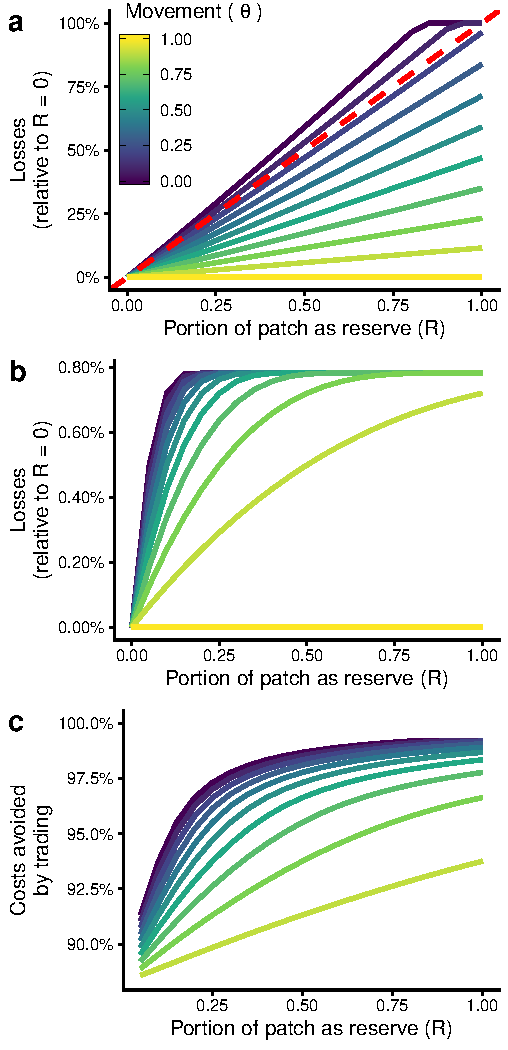
\includegraphics{img/PNA_model.pdf}
\caption{\label{fig:PNA_model}Cost of spatial closures in a vessel-day fishery. Each line represents a possible value of stock movement ($\theta$; line color). The revenue losses to Patch 1 (vertical axis) are relative to a fishery with no spatial closures, and are shown as a function of reserve size ($R$; horizontal axis) and movement (color). Costs are shown for Patch 1 when there is no trading (A) and when trading is allowed (B). Costs avoided by trading are shown in (C). Dashed red line in (A) is a 1:1 line.}
\end{figure}

% Costs of different allocation rules
\begin{figure}[htbp]
\centering
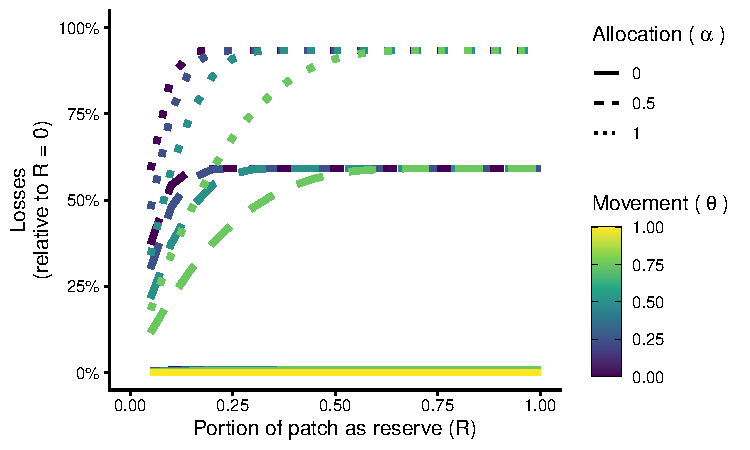
\includegraphics{img/allocation_cost_plot.pdf}
\caption{\label{fig:allocation_cost_plot}Costs of a spatial closure for Patch 1 under different allocation rules. Each line represents the revenue losses for a combination of allocation rules ($\alpha$; line type) and movement ($\theta$; color) for different reserve sizes ($R$; horizontal axis). An effort-based allocation and low movement values result in the highest costs. Cost can be minimized for all movement values if allocation is based on biomass.}
\end{figure}

% Effort redistribution bars for PNA and KIR
\begin{figure}[htbp]
\centering
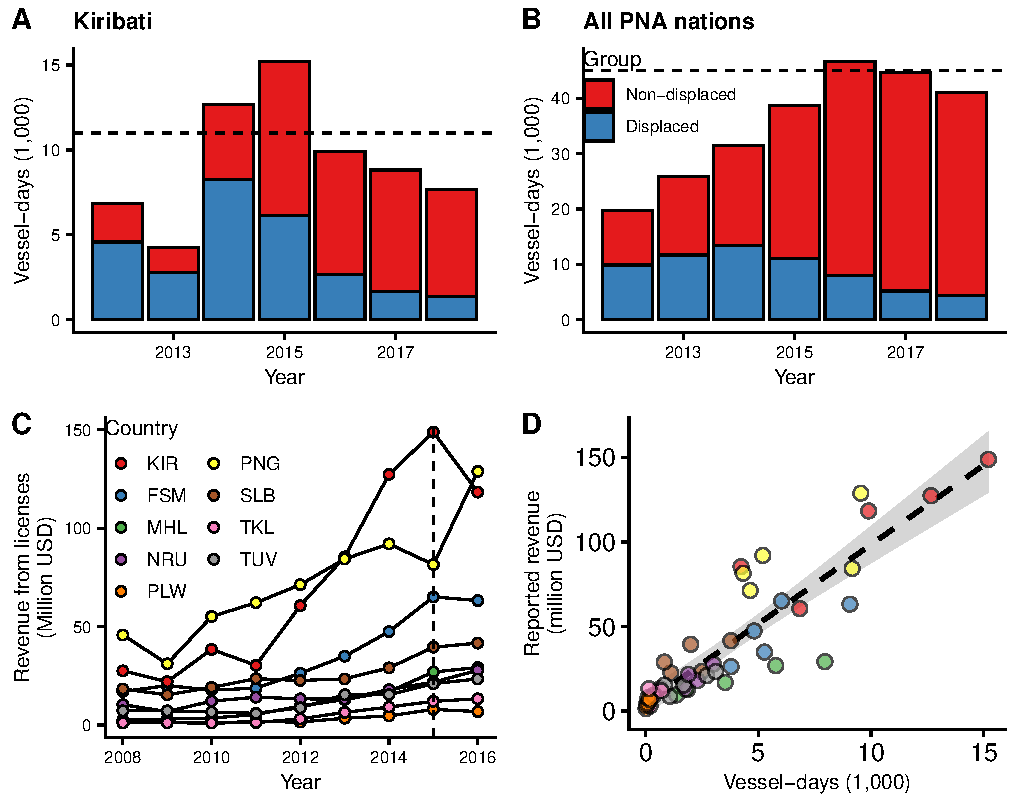
\includegraphics{img/empirical.pdf}
\caption{\label{fig:empirical}Effort displacement and license revenues. Pannels (A) and (B) show AIS-derived annual vessel-days for Kiribati and for all Parties to the Nauru Agreement (PNA). Annual effort is broken down by displaced, non-displaced, and other vessels. The dashed horizontal lines represent the total allowable effort in Kiribati (11,000 days \cite{yeeting2018stabilising}) and the PNA (45,000 days). Pannel (C) shows annual revenue from fishing license fees by country and year (2008 - 2016) and pannel (D) shows the correspondence between FFA-reported revenues and AIS-derived vessel-day observations (2012 - 2016). The dashed line represents line of best fit.}
\end{figure}

% Map of LSMPAS in PNA
\begin{figure}
\centering
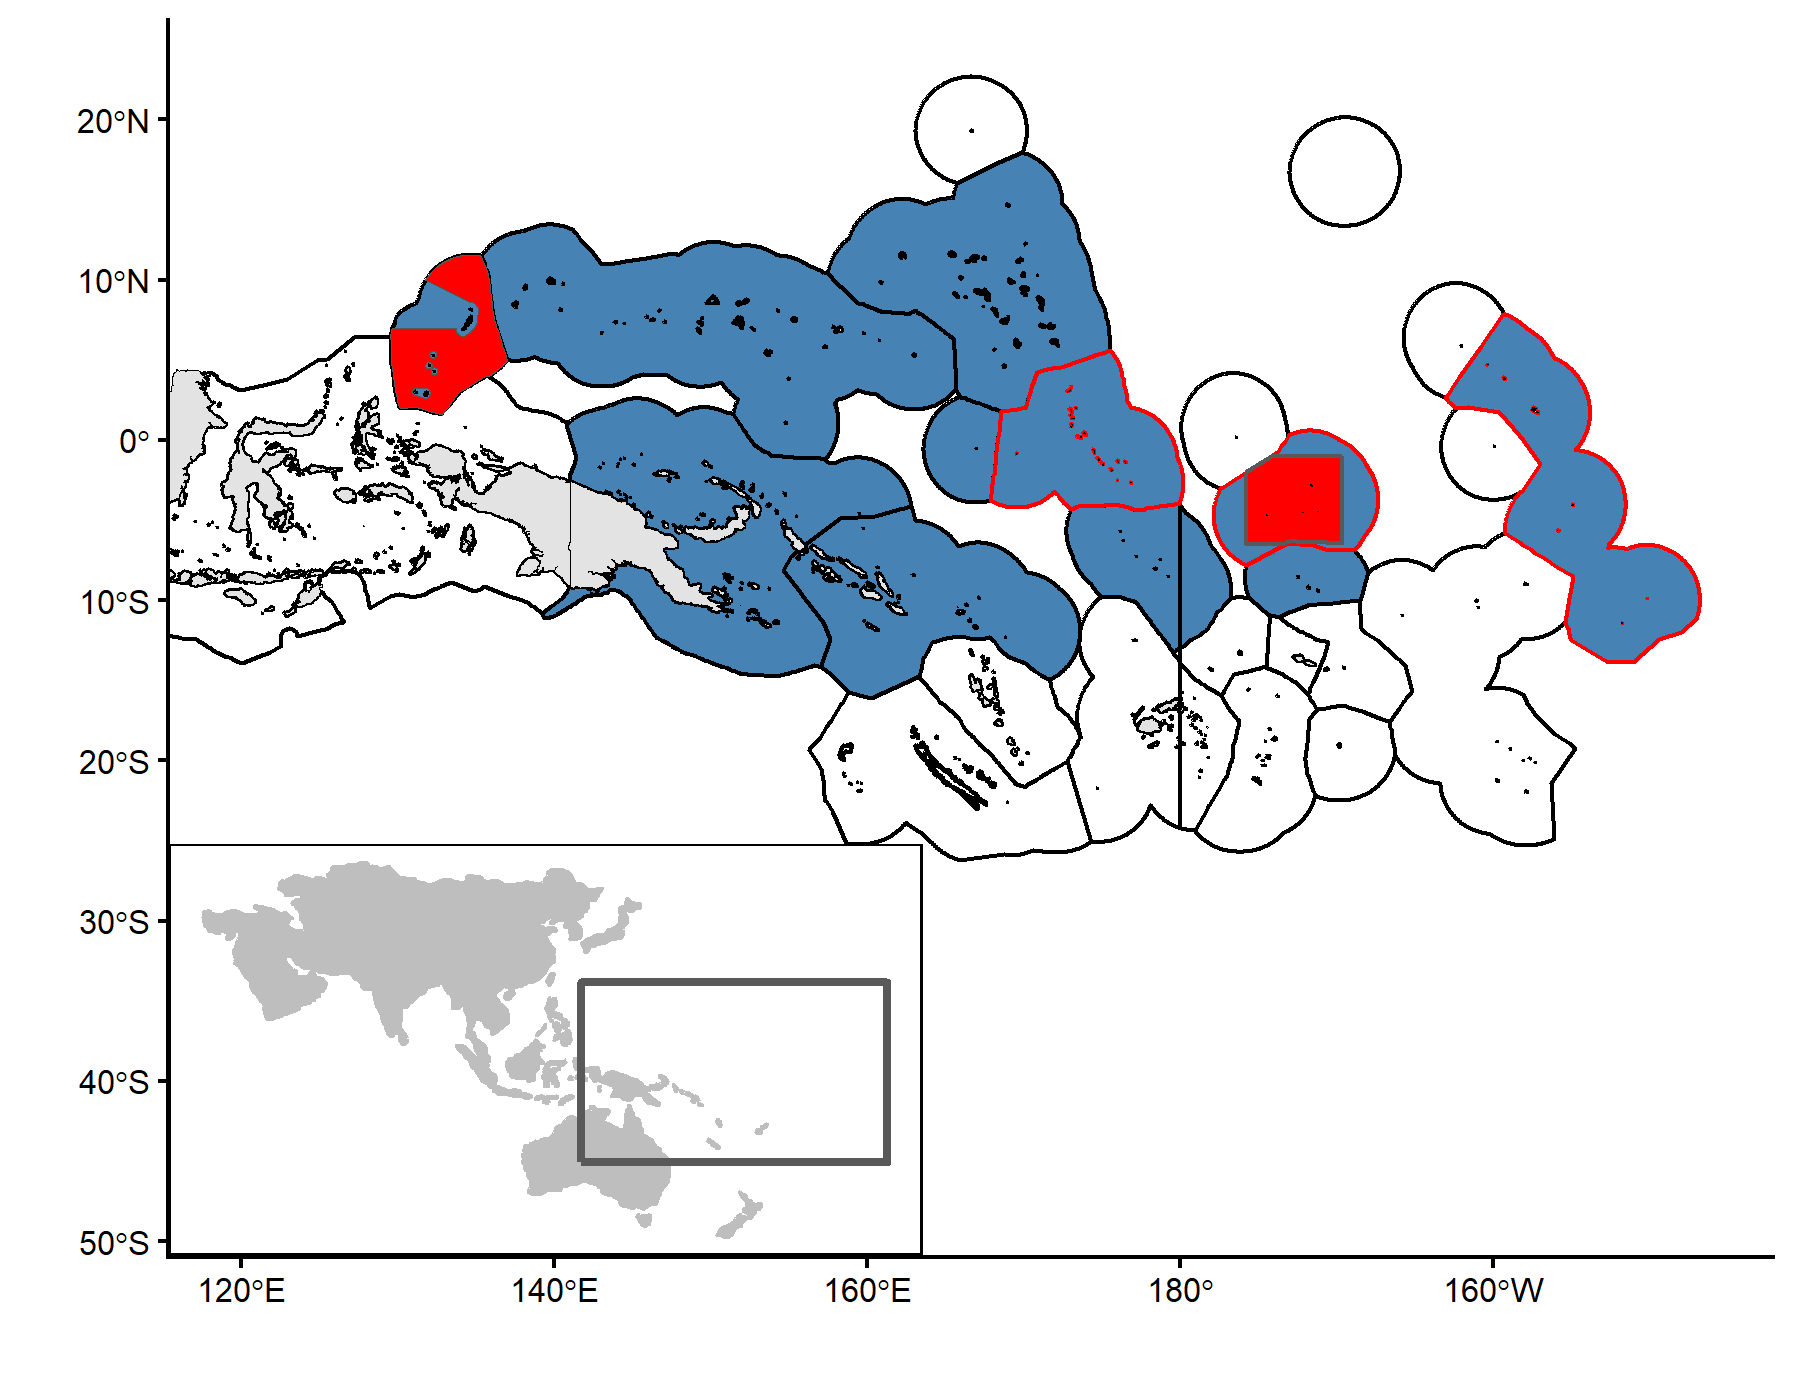
\includegraphics{img/PNA_map.png}
\caption{\label{fig:PNA_map}Map of the Exclusive Economic Zones (EEZs) of the region of interest. Parties to the Nauru Agreement (PNA) are shown in blue, while empty polygons indicate all others. A red line indicates the Kiribati EEZ. The solid red and purple polygons show The Phoenix Islands Protected Area implemented in 2015 and the proposed Palau National Marine Sanctuary. Land masses are shown in gray. Labels indicate ISO3 country codes for PNA members (PLW: Palau, PNG: Papua New Guinea, FSM: Federal States of Micronesia, SLB: Solomon Islands, NRU: Nauru, MHL: Marshal Islands, KIR: Kiribati, TUV: Tuvalu, TKL: Tokelau).}
\end{figure}

\end{document}
